\documentclass[a4paper,11pt]{article}
\usepackage{amsmath,amsthm,amsfonts,amssymb,amscd,amstext,vmargin,graphics,graphicx,tabularx,multicol} 
\usepackage[francais]{babel}
\usepackage[utf8]{inputenc}  
\usepackage[T1]{fontenc} 
\usepackage{pstricks-add,tikz,tkz-tab,variations}
\usepackage[autolanguage,np]{numprint} 

\setmarginsrb{1.5cm}{0.5cm}{1cm}{0.5cm}{0cm}{0cm}{0cm}{0cm} %Gauche, haut, droite, haut
\newcounter{numexo}
\newcommand{\exo}[1]{\stepcounter{numexo}\noindent{\bf Exercice~\thenumexo} : \marginpar{\hfill /#1}}
\reversemarginpar


\newcounter{enumtabi}
\newcounter{enumtaba}
\newcommand{\q}{\stepcounter{enumtabi} \theenumtabi.  }
\newcommand{\qa}{\stepcounter{enumtaba} (\alph{enumtaba}) }
\newcommand{\initq}{\setcounter{enumtabi}{0}}
\newcommand{\initqa}{\setcounter{enumtaba}{0}}

\newcommand{\be}{\begin{enumerate}}
\newcommand{\ee}{\end{enumerate}}
\newcommand{\bi}{\begin{itemize}}
\newcommand{\ei}{\end{itemize}}
\newcommand{\bp}{\begin{pspicture*}}
\newcommand{\ep}{\end{pspicture*}}
\newcommand{\bt}{\begin{tabular}}
\newcommand{\et}{\end{tabular}}
\renewcommand{\tabularxcolumn}[1]{>{\centering}m{#1}} %(colonne m{} centrée, au lieu de p par défault) 
\newcommand{\tnl}{\tabularnewline}

\newcommand{\trait}{\noindent \rule{\linewidth}{0.2mm}}
\newcommand{\hs}[1]{\hspace{#1}}
\newcommand{\vs}[1]{\vspace{#1}}

\newcommand{\N}{\mathbb{N}}
\newcommand{\Z}{\mathbb{Z}}
\newcommand{\R}{\mathbb{R}}
\newcommand{\C}{\mathbb{C}}
\newcommand{\Dcal}{\mathcal{D}}
\newcommand{\Ccal}{\mathcal{C}}
\newcommand{\mc}{\mathcal}

\newcommand{\vect}[1]{\overrightarrow{#1}}
\newcommand{\ds}{\displaystyle}
\newcommand{\eq}{\quad \Leftrightarrow \quad}
\newcommand{\vecti}{\vec{\imath}}
\newcommand{\vectj}{\vec{\jmath}}
\newcommand{\Oij}{(O;\vec{\imath}, \vec{\jmath})}
\newcommand{\OIJ}{(O;I,J)}


\newcommand{\reponse}[1][1]{%
\multido{}{#1}{\makebox[\linewidth]{\rule[0pt]{0pt}{20pt}\dotfill}
}}

\newcommand{\titre}[5] 
% #1: titre #2: haut gauche #3: bas gauche #4: haut droite #5: bas droite
{
\noindent #2 \hfill #4 \\
#3 \hfill #5

\vspace{-1.6cm}

\begin{center}\rule{6cm}{0.5mm}\end{center}
\vspace{0.2cm}
\begin{center}{\large{\textbf{#1}}}\end{center}
\begin{center}\rule{6cm}{0.5mm}\end{center}
}



\begin{document}
\pagestyle{empty}
\titre{TP : Droite d'Euler}{Nom :}{Prénom :}{Classe}{Date}


\vspace*{1cm}

\q Construire un triangle quelconque ABC.\\

\q Placer les milieux des côtés [AB], [AC] et [BC]. Les renommer pour les appeler I, J et K.\\

\q Construire les 3 médianes du triangle ABC. Les colorier en vert. Elles se coupent en D.\\

\q Construire les 3 hauteurs du triangle ABC. Les colorier en bleu. Elles se coupent en E.\\

\q Construire les 3 médiatrices du triangle ABC. Les colorier en noir. Elles se coupent en F.\\

\q Tracer la droite qui passe par D et E. La colorier en rouge (épaisseur du trait 3). Que remarque-t-on ?\\

\reponse[2]\\

\q Déplacer les points A, B ou C. Quelle conjecture pouvez-vous faire sur les points D, E et F ?\\


Conjecture : \reponse[2] \\


\vspace*{1cm}
\begin{center}
\includegraphics[scale=1]{droiteeuler.eps} 

\end{center}

\begin{center}
\textbf{Évaluation  durant le TP :}
\end{center}

\begin{center}
\begin{tabular}{|c|c|}
\hline 

Triangle ABC  & \hspace*{1cm}/1 \\ 

\hline 
Médianes & \hspace*{1cm}/2 \\ 
\hline 
Hauteurs & \hspace*{1cm}/2 \\ 
\hline 
Médiatrices & \hspace*{1cm}/2 \\ 
\hline 
Droite & \hspace*{1cm}/1 \\ 
\hline 
Conjecture & \hspace*{1cm}/2 \\ 
\hline 
\end{tabular} 
\end{center}



\begin{flushright}
\textbf{Note : ......./ 10 }
\end{flushright}

 
\newpage

\pagestyle{empty}
\titre{TP : Théorème de Napoléon}{Nom :}{Prénom :}{Classe}{Date}


\vspace*{1cm}


\initq \q Construire un triangle quelconque ABC.\\

\q A l’extérieur de celui-ci, construire trois triangles équilatéraux ABM, BCN et ACP.\\

\q Dans chacun de ces trois triangles, construire deux médianes.\\

\qa Dans le triangle ABM, les deux médianes se coupent en I.\\

\qa Dans le triangle BCN, les deux médianes se coupent en J.\\

\qa Dans le triangle ACP, les deux médianes se coupent en K.\\

\q Tracer le triangle IJK.\\

\q Déplacer les points A, B ou C. Quelle semble être la nature du triangle IJK ?\\
(On pourra afficher les longueurs IJ, JK et IK)


Conjecture : \reponse[2]\\

\vspace*{1cm}

\begin{center}
\textbf{\includegraphics[scale=1]{napoleon.eps} 
}\end{center}




\begin{center}
\textbf{Évaluation  durant le TP :}
\end{center}

\begin{center}
\begin{tabular}{|c|c|}
\hline 
Médianes & \hspace*{1cm}/2 \\ 
\hline 
Trois triangles équilatéraux & \hspace*{1cm}/2 \\ 
\hline 
Deux médianes & \hspace*{1cm}/2 \\ 
\hline 
Triangle IJK & \hspace*{1cm}/2 \\ 
\hline 
Nature du triangle IJK & \hspace*{1cm}/2 \\ 
\hline 
\end{tabular} 
\end{center}



\begin{flushright}
\textbf{Note : ......./ 10 }
\end{flushright}


\end{document}
